\documentclass[11pt,a4paper]{article}

\usepackage[utf8]{inputenc}
\usepackage[T1]{fontenc}
\usepackage[a4paper,margin=1in]{geometry}
\usepackage{amsmath,amssymb,amsfonts}
\usepackage{booktabs,array,longtable}
\usepackage{graphicx}
\usepackage{xcolor}
\usepackage{listings}
\usepackage[inline]{enumitem}
\usepackage{hyperref}
\usepackage{setspace}
\usepackage{fancyhdr}
\usepackage{titlesec}

\definecolor{tumblue}{RGB}{0,101,189}
\hypersetup{colorlinks=true, linkcolor=tumblue, urlcolor=tumblue}

\setstretch{1.08}
\setlength{\parindent}{0pt}
\setlength{\parskip}{0.6em}

\pagestyle{fancy}
\fancyhf{}
\setlength{\headheight}{14pt}
\lhead{Assignment 5}
\rhead{Layout Optimization for LCoE}
\cfoot{\thepage}

\titleformat{\section}{\large\bfseries}{\thesection.}{0.5em}{}
\titleformat{\subsection}{\normalsize\bfseries}{\thesubsection}{0.5em}{}

\definecolor{codegray}{RGB}{248,248,248}
\definecolor{codeborder}{RGB}{220,220,220}

\lstdefinestyle{mystyle}{
	backgroundcolor=\color{codegray},
	frame=single,
	rulecolor=\color{codeborder},
	basicstyle=\ttfamily\small,
	breaklines=true,
	columns=fullflexible,
	keepspaces=true,
	showstringspaces=false,
	tabsize=4
}
\lstset{style=mystyle}

\title{\textbf{Assignment 5}\\
	\normalsize Layout Optimization for LCoE}
\author{Chinmay S Patil}
\date{}

\graphicspath{{./}}
\begin{document}

%% -------------------------------------------------------
%%  TITLE BLOCK
%% -------------------------------------------------------
\begin{center}
    {\LARGE\bfseries Assignment 5: Layout Optimization for LCoE}\\[0.4em]
    {\large Praktikum Design of Wind Farms\quad|\quad TU München}\\[0.2em]
    {\normalsize Wind Energy Institute\quad|\quad Prof.\ Dr.\ Carlo L.\ Bottasso}\\[0.2em]
    {\small Dr.\ sc.\ Hadi Hoghooghi \quad|\quad MSc.\ Samuel Kainz}
\end{center}

\vspace{1em}
\hrule
\vspace{1.5em}

%% -------------------------------------------------------
%%  TASK 1
%% -------------------------------------------------------
\section{Task 1: Wind Rose at Hub Height}

Wind speed and direction data were downloaded from the New European Wind Atlas (NEWA)
for Marienplatz, Munich, covering the mesoscale time series from 1989 to 2022.
The raw data were provided at 10\,m height and scaled to hub height (120\,m) using the
power-law wind shear model with exponent $\alpha = 0.20$:

\begin{equation}
    U(h) = U_{\text{ref}}\left(\frac{h}{h_{\text{ref}}}\right)^{\alpha}
\end{equation}

\subsection{Wind Rose}

\begin{figure}[h!]
    \centering
    
\includegraphics[width=0.62\textwidth]{wind_rose.png}
    \caption{Wind rose at Marienplatz, Munich -- NEWA Mesoscale Time Series 1989--2022
             (hub height 120\,m, mean wind speed = 6.58\,m/s).}
    \label{fig:windrose_task1}
\end{figure}

The wind rose in Figure~\ref{fig:windrose_task1} shows a strongly dominant westerly and
south-westerly wind regime, with wind speeds of 6--9\,m/s (orange) and 9--12\,m/s (salmon)
being most frequent. Higher wind speeds above 15\,m/s (purple) also arrive predominantly
from the west. Wind activity from the north and south is negligible. The mean wind speed
at hub height is \textbf{6.58\,m/s}.

This directionality is a critical input for the layout optimisation in Task~3: turbines
aligned in the west--east direction will experience the largest wake losses under the
prevailing wind.

%% -------------------------------------------------------
%%  TASK 2
%% -------------------------------------------------------
\section{Task 2: Baseline Wind Farm Evaluation}

The initial layout places eight IEA 3.4\,MW turbines in a $4 \times 2$ grid centred within
the 2.8\,km\,$\times$\,2.8\,km boundary. Wake interactions were evaluated with the
Gauss wake model (default parameters) in FLORIS.

\subsection{Results}

\begin{table}[h!]
    \centering
    \caption{Baseline wind farm performance metrics.}
    \label{tab:baseline}
    \begin{tabular}{lcc}
        \toprule
        \textbf{Parameter} & \textbf{Value} & \textbf{Unit} \\
        \midrule
        AEP                  & 68.36  & GWh/yr  \\
        Capacity Factor      & 28.95  & \%      \\
        Farm Efficiency      & 77.62    & \%      \\
        LCoE                 & 62.40  & \$/MWh  \\
        PI                   & 0.1194  & --  \\
        \bottomrule
    \end{tabular}
\end{table}

Because the turbines are aligned east--west and dominant winds come from the west, the
rear row suffers substantial wake losses from the front row, reducing AEP and farm
efficiency. The baseline LCoE of $\sim$62.4\,\$/MWh exceeds the electricity price of
67\,\$/MWh; however, because LCoE\,$<$\,electricity price, profitability is borderline.
The layout has clear room for improvement through optimisation.

%% -------------------------------------------------------
%%  TASK 3
%% -------------------------------------------------------
\section{Task 3: COBYLA Layout Optimisation}

The \texttt{scipy.optimize.minimize} function with the \textbf{COBYLA} (Constrained
Optimization BY Linear Approximation) gradient-free method was used to optimise the
16 turbine coordinates ($8\times x$, $8\times y$) so as to minimise the LCoE of the
wind farm. The following constraints were enforced:

\begin{itemize}
    \item All turbines must remain within the 2.8\,km\,$\times$\,2.8\,km boundary.
    \item Minimum turbine separation of $2D = 260$\,m between all pairs.
\end{itemize}

\newpage

\subsection{Convergence}

\begin{figure}[h!]
    \centering
    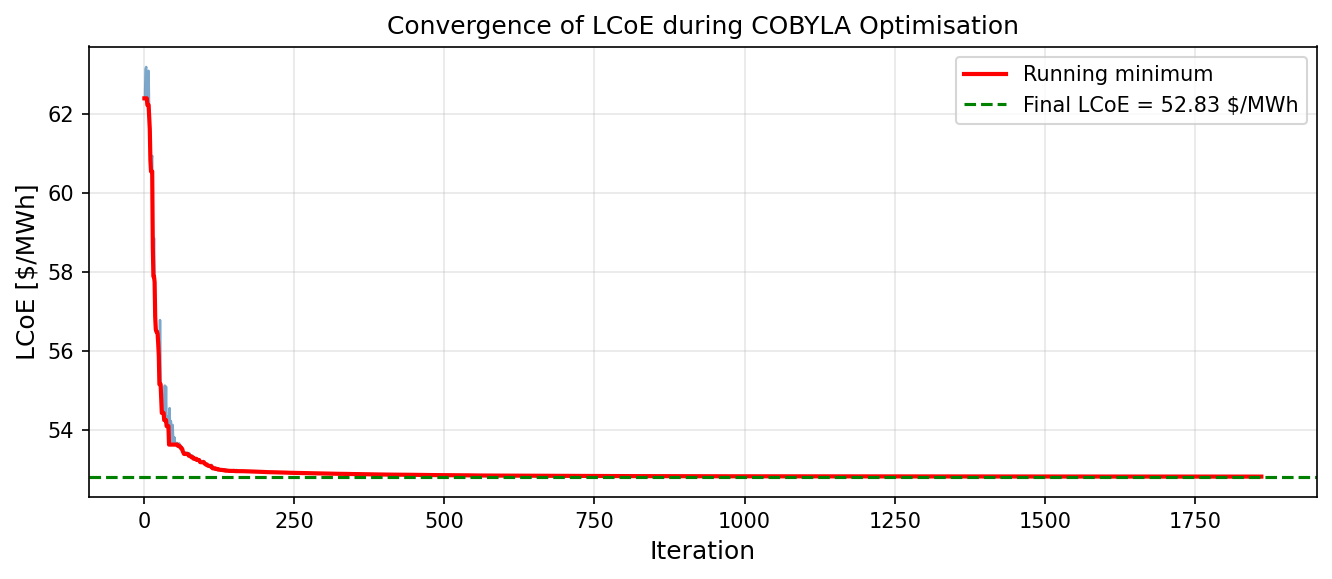
\includegraphics[width=\textwidth]{task3_convergence.png}
    \caption{Convergence of LCoE during COBYLA optimisation.
             The running minimum (red) drops rapidly within the first 250 iterations
             and flattens at the final optimum of 52.83\,\$/MWh (green dashed line).}
    \label{fig:convergence}
\end{figure}

\begin{figure}[h!]
    \centering
    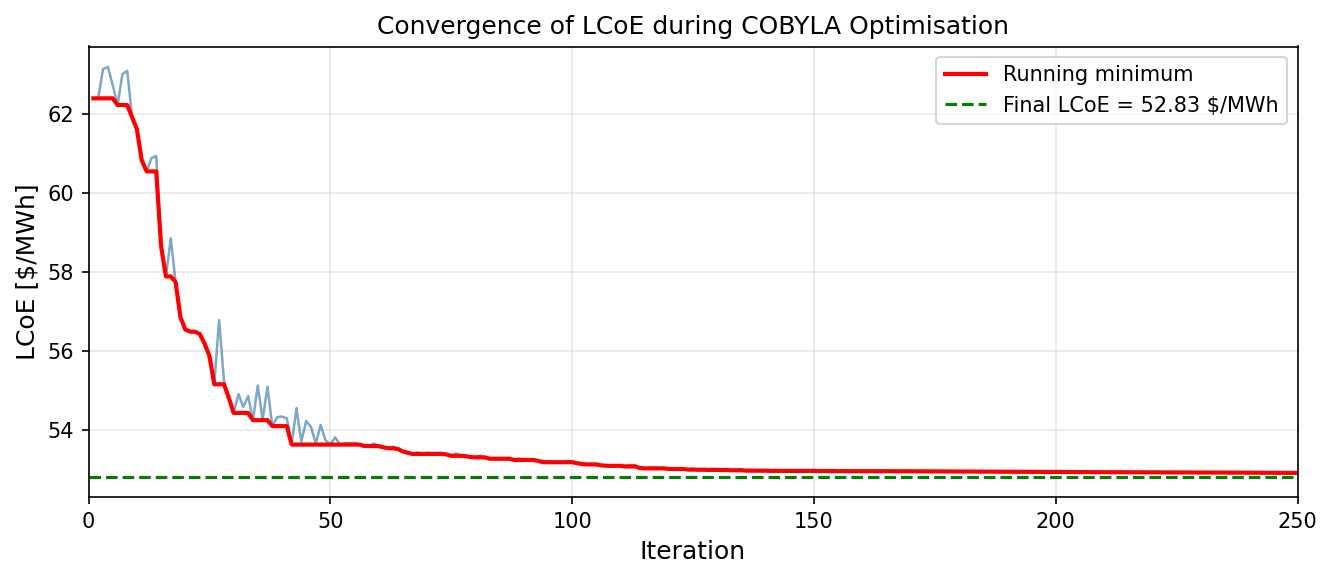
\includegraphics[width=\textwidth]{task3_convergence_truncated.png}
    \caption{Truncated graph of Convergence of LCoE during COBYLA optimisation.}
    \label{fig:convergence_truncated}
\end{figure}

Figure~\ref{fig:convergence} shows the running minimum LCoE over 1900 iterations.
The optimiser starts at approximately 63\,\$/MWh and converges rapidly, with the
objective essentially flat after iteration 250, confirming that a local optimum
has been reached.

\newpage

\subsection{Optimised Layout}

\begin{figure}[h!]
    \centering
    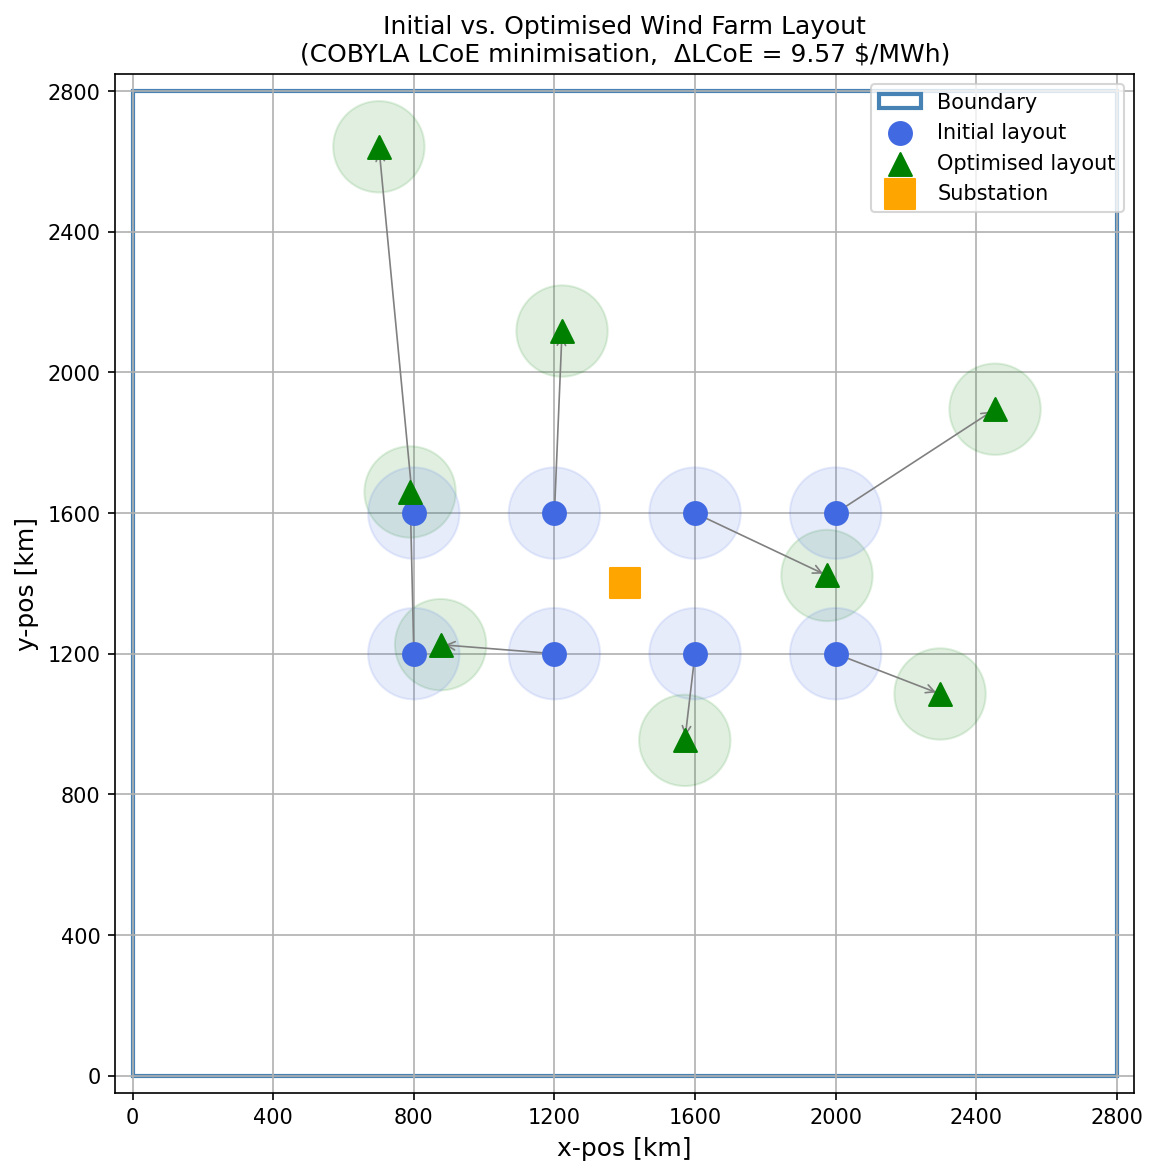
\includegraphics[width=0.75\textwidth]{task3_layout.png}
    \caption{Initial (blue circles) vs.\ optimised (green triangles) wind farm layout.
             Arrows indicate turbine displacement. $\Delta\text{LCoE} = 9.57$\,\$/MWh.}
    \label{fig:layout}
\end{figure}

The optimised layout (Figure~\ref{fig:layout}) shows several key changes relative to
the baseline:

\begin{itemize}
    \item Turbines that were clustered in the west--east direction have been spread in
          the north--south direction, reducing wake overlap under the dominant westerly wind.
    \item Several turbines moved towards the boundary edges to maximise mutual separation.
    \item All minimum spacing constraints ($2D = 260$\,m) are satisfied, as confirmed by
          the non-overlapping exclusion circles.
\end{itemize}

\subsection{Comparison of Results}

\begin{table}[h!]
    \centering
    \caption{Performance comparison: initial vs.\ optimised layout.}
    \label{tab:comparison}
    \begin{tabular}{lccc}
        \toprule
        \textbf{Parameter} & \textbf{Initial} & \textbf{Optimised} & \textbf{Unit} \\
        \midrule
        AEP              & 68.36 & 87.28 & GWh/yr \\
        Capacity Factor  & 28.95 & 36.96 & \%     \\
        Farm Efficiency  & 77.62   & 99.11   & \%     \\
        LCoE             & 62.40 & 52.83      & \$/MWh \\
        $\Delta$LCoE     & \multicolumn{2}{c}{9.5731} & \$/MWh \\
        PI             & 0.1194 & 0.4624      & \$/MWh \\
        \bottomrule
    \end{tabular}
\end{table}

\subsection{Profitability Discussion}

The optimised LCoE of \textbf{52.83\,\$/MWh} is below the electricity price of
67\,\$/MWh, confirming that the project has become clearly profitable after optimisation.
The $\Delta\text{LCoE}$ of 9.57\,\$/MWh was achieved purely by repositioning turbines,
without any additional capital expenditure.

The improvement in farm efficiency from 77.62\,\% to 99.11\,\% demonstrates
that wake losses were substantially reduced. This highlights layout optimisation as a
highly cost-effective measure to improve wind farm economics -- a finding consistent with
the strongly directional wind resource observed at the Munich site.

\end{document}